\documentclass[12pt]{article}
\usepackage{graphicx}
\usepackage{Style-Thesis-Report}

% You can define your own commands like this
\newcommand{\um}{$\upmu$m} % easily creates the label for ``micrometers''t

\begin{document} % Here is where the document begins
	
\begin{titlepage} 
\thispagestyle{empty}
	\begin{center}
	
		\begin{picture}(50,50)
\put(-20,-20){\hbox{
\includegraphics[scale=0.06]{Figures/McGill}}}
\end{picture}
\Huge
\textsc{McGill Physical Journal}
		\begin{picture}(50,50)
\put(10,-20){\hbox{
\includegraphics[scale=0.06]{Figures/atom}}}
\end{picture}
		\vspace*{1.5cm}
		
		\Huge
		\textbf{Direct observation of meow meow in the presence of meow}
		\large
		\vspace{1.5cm}
		
		First Author (StudentID), Second Author (Student ID), Third Author (Student ID)
	  % Add your names and student ID here
		
		McGill University Department of Physics
		
		\today
	\end{center}
		\hrule
	\begin{abstract} % This is the abstract. Replace the content with your own wording.
This file is already set up with the correct margins, font, and line spacing. It is designed to show examples of how to create and organize a LaTeX document. Simply make a copy of this tex file and then overwrite all of the nonsense with your own content. If this gives you trouble, or you're just annoyed with LaTeX, Jack Sankey highly recommends using LyX instead. LyX is based on latex, but you don't have to look at the underlying code (though you can if you want!). This means everything you learn and do in LyX (especially equations!) will be easier, and can be directly applied / copied / pasted to a latex document, should you go this route in the future. If you stick with LaTeX, Jack Sankey can say from experience that TeXstudio is the best editor he has seen. I (T.B.) started using TeXnicCenter when I was an undergraduate student and have used it since then. If you are collaborating with peers you might also want to check out overleaf. You can find this template also online at \href{https://www.overleaf.com/read/djxgtnvnwgkp}{OverLeaf}.
\end{abstract}
\hrule
\end{titlepage}
%\tableofcontents{}
%\thispagestyle{empty}
%\pagebreak
\setcounter{page}{1}
%The following commands will define header and footer
\rhead{McGill Physical Journal} % Do not change!
\lhead{Lab title}  % Add your lab title here
\cfoot{Page \thepage} % Do not change

\section{Introduction}\label{sec:introduction}
This section outlines basic goal of the experiments and the relevant theory used for interpreting/analysing the results should appear first in the main body of the report. The purpose of the Introduction is to present the background information, basic concepts and equations required by the reader to understand i) the purpose of the experiment and ii) the methods used in treating the data. 

It serves little purpose, and is not considered good practice, to rewrite or copy large portions from notes, the lab manual or texts. Furthermore, derivations of equations given elsewhere should not be reproduced. If the derivation is of particular interest reference can be made to the appropriate source or it can be placed in an appendix. However, a brief presentation of basic theory, with relevant equations, in the words and style of the author is essential.  	
%
See additional information on this and other sections in the lecture notes and at \href{http://www.nature.com/scitable/ebooks/english-communication-for-scientists-14053993/contents}{\textsc{Nature}}.

You can write a section intro here. Section \ref{sec:sub} below shows a demo of a subsection.

This is a new paragraph, with some $M_\textrm{ath}=I_n lin_e$, and a larger equation can be made as follows:
%
\begin{equation}\label{eq:pants}
ax^2 + bx + c = 0
\end{equation}
%
Sadly, Eq.~\ref{eq:pants} is super boring. Note the little \% symbols in the latex code. They prevent a new paragraph from forming. An empty line in your latex document will be interpreted as new paragraph with the first word indented. 

\subsection{Test Subsection}\label{sec:sub}
You can also do subsubsections if you really want. 

\begin{figure}
	%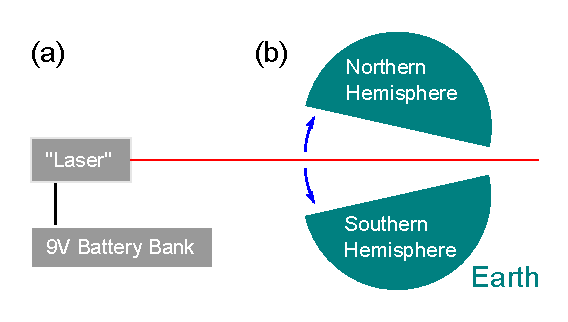
\includegraphics[width=12cm]{Figures/Figure1}
	%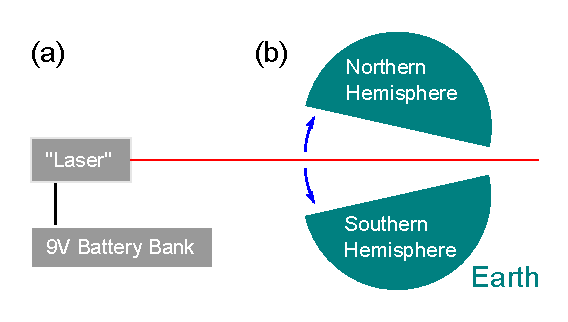
\includegraphics[width=0.8 \textwidth]{Figures/Figure1}%% This is a different way to scale a figure to size
	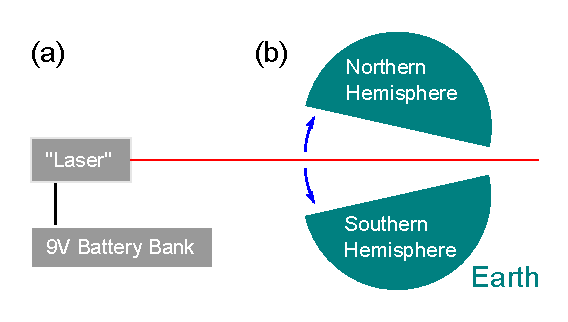
\includegraphics[scale=0.9]{Figures/Figure1}%% Yet another way to scale the figure to size
	\caption{Space Laser Facility and action upon earth. (a) Space laser facility: A bank of $10^{18}$ 9V batteries powers the primary laser. (b) The laser output is swept along the equator from east to west at a rate of 5 radians / hour, producing a clean split between the northern and southern hemispheres. }
	\label{fig:laser}
\end{figure}

Figure \ref{fig:laser}(a) shows a simplified drawing of the Space Laser Facility (SPL). A bank of $10^{18}$ 9-volt batteries (Eveready \textregistered X-treme bulkbox) supplies power to a sophisticated heat beam known as a ``Laser''. In Fig.~\ref{fig:laser}(b), we show the estimated response of earth for a laser swept along the equator at a rate of 5 radians / hour from east to west. Blue arrows indicate the approximate direction of motion. Due to the rotation of the earth, a similar sweep from west to east will not produce a clean cut \cite{Sankey2010Strong}. The wavelength of this laser, $\lambda=1.55$ \um, is chosen primarily because the telecom industry has produced a multitude of low-cost components at this wavelength.

We definitely recommend using Mendeley to organize your citations and generate a bibliography file. You can set this up so that from the abstract page online, you can click a button that adds it to your library. Then it's just a matter of exporting to ``bibtex'' format.

\subsection{Tables in \LaTeX}\label{sec:tables}
In subsection \ref{sec:tables} we shall present a table to introduce the table environment. Table~\ref{tab:TITANEC} is copied from the manuscript of \cite{Brunner2013}.
\begin{table}
	\caption{\label{tab:TITANEC}Ion bunch intensities derived from the measured $^{124\textnormal{g,m},126}$Cs photopeak intensities and the duration of each time slice (TS). The value marked with $^{\dagger}$ was measured with $\Delta t_{meas}=\Delta t_{BGND}=50$\,ms. All other measurements were performed with 25\,ms.}
	\centering
		\begin{tabular}{rccc}
			Isotope&TS&Duration [h]&Ion bunch intensity\\
			  \hline\noalign{\smallskip}
			$^{124\textnormal{m}}$Cs&&\multirow{2}{*}{6}&$4.48(63)\cdot10^3$\\
			$^{124\textnormal{g}}$Cs&&&$1.34(13)\cdot10^5$\\
			$^{126}$Cs&1&3&$2.65(32)\cdot10^5\ ^{\dagger}$\\
			$^{126}$Cs&2&1&$2.54(54)\cdot10^5$\\
			$^{126}$Cs&3&2&$1.85(46)\cdot10^5$\\
			$^{126}$Cs&4&3&$1.80(32)\cdot10^5$\\
			$^{126}$Cs&5&3&$1.61(30)\cdot10^5$\\
			\noalign{\smallskip}\hline
		\end{tabular}
\end{table}

\section{Materials and Methods}
Maximum $\approx500$ words.  Maximum 2 Figures.

A description of the equipment and procedures used to make the measurements are given in this section. When special apparatus is used, a description of the operating principles together with a clearly labelled schematic diagram is desirable. 

 	Experimental procedure should include a concise outline of the actual procedure, which should differ somewhat from that described in the notes or elsewhere. This section should NOT be a detailed transcription of the manual or take the form of a \textit{recipe}; e.g. “and then we pressed ‘setup 2’ on the oscilloscope, and then moved the cursor to measure the position of...”. Instead, it should be a very concise outline of the main points of the procedure sufficient to convey a clear overview of the experimental procedure to the reader. This outline should consist of concise factual statements, e.g., "The heat capacity of the calorimeter and contents were determined by measuring the temperature change that resulted from the addition of a known quantity of heat". 

\section{Results}
Maximum 500 words. Use the minimum number of Figures and Tables necessary to fully present your results. 

This section presents the experimental data and the results of any analyses including the estimation of experimental uncertainties.  Your results should be presented in a logical sequence.  Do not jump around in an inconsistent, hard to follow manner. Any assumptions made in the treatment of data should be clearly specified.  The reader should be informed, using explanatory sentences how the raw data obtained in the laboratory were transformed into the desired results; i.e. your graphs and tables should appear in this section, but this section is not ONLY your graphs and tables.    

\section{Discussion}
Maximum 500 words. Use the minimum number of Figures and Tables necessary to fully discuss your results. 

The Discussion evaluates whether or not the experiment objectives have been met (i.e. was the experiment a success) and what the results actually mean. This portion of the report allows some freedom, but the purpose is to explain the significance/meaning of the results to the reader; i.e. to ‘interpret’ the results.  
In the discussion section, important features of the results should be highlighted. Comparison should be made with accepted values if relevant and available.  This comparison gives an estimate of the accuracy of the experiment and provides an opportunity to assess different methods (i.e. those you used and those others have used) and to comment on your error analysis. Do the results obtained in this experiment agree - within quoted uncertainty - of accepted values? If there is a discrepancy, by how many standard deviations?  Why? 
What (if any) is the theoretical significance of the results? The Discussion should include a clear, concise presentation of how the results demonstrate key concepts or impact on questions of theoretical importance. Any direct questions asked of you in the lab manual should also be addressed in this section.

\section{Conclusions}
Maximum 300 words.

In the Conclusion section, state the most important outcome of your work. Do not simply summarize the points already made in the body — instead, interpret your findings at a higher level of abstraction. Show whether, or to what extent, you have succeeded in addressing the need stated in the Introduction. At the same time, do not focus on yourself (for example, by restating everything you did). Rather, show what your findings mean to readers. Make the Conclusion interesting and memorable for them. 
At the end of your Conclusion, consider including perspectives — that is, an idea of what could or should still be done in relation to the issue addressed in the paper. If you include perspectives, clarify whether you are referring to firm plans for yourself and your colleagues ("In the coming months, we will . . . ") or to an invitation to readers ("One remaining question is \dots ").
\bibliographystyle{IEEEtran}
\bibliography{MyBibliography}
%%%%%%%%% The appendix starts here. You can add tables, pictures, plots, graphs, data sets to your appendix.
\newpage
\appendix
\section{First Appendix}
All the information that is required to follow your work but that is too detailed for the main text.
\section{Second Appendix}
One of the best introductions to \LaTeX$2_{\epsilon}$  is the \href{http://www.ctan.org/tex-archive/info/lshort/}{not too short introduction to \LaTeX}.
\section{Third Appendix}
Your work will likely build on, rely on, or otherwise make use of the results or work of others.  In all such cases it is essential that you properly ‘reference’ the appropriate original source.  References should be numbered consecutively in order of first appearance throughout the text. Software is available to the McGill community to make this very easy (EndNote for Window/Word, BibTeX for LaTeX) which is available to all McGill students.  References to Web URL’s are to be discouraged but are sometimes necessary.

\textbf{If you state a fact that is based on someone else's research or work you MUST cite it!}
\end{document}
%%%%%%
% McGil logo from McGill webpage
% Note: atom logo from http://images.google.de/imgres?imgurl=https%3A%2F%2Fupload.wikimedia.org%2Fwikipedia%2Fcommons%2Fthumb%2F8%2F80%2FAtom_editor_logo.svg%2F2000px-Atom_editor_logo.svg.png&imgrefurl=https%3A%2F%2Fcommons.wikimedia.org%2Fwiki%2FFile%3AAtom_editor_logo.svg&h=1832&w=2000&tbnid=Pu9l8_1ca47MzM%3A&vet=1&docid=DMy5AX000LwZRM&ei=bmZqWO-xL-mRgAaFlrGgCw&tbm=isch&iact=rc&uact=3&dur=2247&page=0&start=0&ndsp=18&ved=0ahUKEwjvoP_L2KPRAhXpCMAKHQVLDLQQMwgcKAIwAg&safe=off&bih=634&biw=1141